\chapter{State of the Art}
\label{ch:state-of-the-art}

In this chapter we describe the state of the art of recommender systems.\\
In the first section we start from the basic principles of recommender systems, describing their elementary properties.\\
After that, in the second section, we cover the standard techniques, such as content-based, collaborative and hybrid recommender systems.\\
In the third and fourth sections, we cover the matrix factorization model and factorization machines.\\
The fifth section covers the basic properties and usage of datasets.\\
The sixth section describes evaluation metrics and their use cases.\\
In the seventh sections we describe the main clustering techniques and their use in recommender systems.\\
Finally, in the eighth section we describe the state of the art of knowledge transfer techniques used in recommender systems.



\section{Basic Principles of Recommender Systems}

In this section we start by providing a brief definition of recommender systems and the problems they are faced with.
The most accurate definition of modern recommender systems can be found in Burke's statement:
\begin{displayquote}[Burke, 2002 \cite{10.1007/s10844-018-0530-7}]
\enquote{Any system that produces individualized recommendations as output or has the effect of guiding the user in a personalized way to interesting or useful objects in a large space of possible options.}
\end{displayquote}


\subsection{Recommender Systems Tasks}

While recommender systems in general are aiming at learning and anticipate user preferences to provide helpful suggestions, they are faced with two distinct tasks: items ranking and items ratings prediction.\\
Ranking is the task of selecting from the whole catalog a small number of items to be recommended for each user. We can distinguish two slightly different scenarios for the ranking task. If an item of the catalog can be interacted with multiple times, every item should be eligible for recommendation. For example, in a music streaming service, users usually listen to the same song several times. On the contrary, if users are not expected to choose the same item twice, already rated or seen items are excluded from the items the recommender system suggests.\\
Rating prediction consists in providing a computed rating for each user unrated item. Since items with predicted ratings can then be ordered and selected for ranking, most of the times the two tasks share some characteristics, while the main differences between them are identified in the evaluation test set, evaluation procedure and metrics.


\subsection{Types of Feedback}

Since recommender systems can leverage historical data and user profiles, it is important to distinguish two types of feedback.\\
Explicit feedback are clear and numerical values of how much a user liked or disliked an item he interacted with. While explicit feedback is the most accurate indicator of user preferences and, for this reason, it makes the recommendation task easier, they are usually hard to obtain from users, since a user input is required. Additionally, explicit feedback can easily be user biased, as different users could value a numeric rating differently.\\
Implicit feedback is identified as the user interaction with an item. For example, the action of listening to a song on a streaming service is considered implicit feedback.
Implicit feedback cannot differentiate between positive and negative feedback and as such it is always available but considered less reliable than explicit ratings.


\subsection{Data Structures}

Recommender systems often make use of common data structures, which can be identified in the following matrices:
\begin{itemize}
\item \textbf{User-Content Matrix (UCM)}: given a set of users $U$ and a set of user features $C$, the UCM is a matrix with shape $\abs{U} \times \abs{C}$ where each row represents a user $u \in U$ and each column represents a feature $c \in C$. Each cell $(u,c)$ represents the value of feature $c$ of the user $u$. It can be a real, integer or binary value depending on the nature of the feature. For example, to describe the user age, we could either have a single integer feature, where each cell value would represent the age of the user, or multiple binary features representing different age brackets, where each cell value would be:
\begin{equation*}
(u,l)=
\begin{cases}
0, & \text{if}\ u\ \text{belongs to the age bracket}\ l\\
1, & \text{otherwise}
\end{cases}
\end{equation*}
The approach of splitting a numerical feature into multiple categorical features is called one-hot encoding.\\
The UCM is generally built in content based recommendation approaches.
\item \textbf{Item-Content Matrix (ICM)}: ggiven a set of items $I$ and a set of item labels $L$, the ICM is a matrix with shape $\abs{I} \times \abs{L}$ where each row represents an item $i \in I$ and each column represents a label $l \in L$. Each cell $(i,l)$ represents the value of label $l$ of the item $i$. It can be a real, integer or binary value depending on the nature of the label.\\
Similarly to the UCM, the ICM is generally built in content based recommendation approaches.
\item \textbf{Similarity Matrix}: given a set of users $U$, the user similarity matrix is a matrix with shape $\abs{U} \times \abs{U}$, where each row $u_r$ and column $u_c$ represent users $u \in U$ and each cell represents the similarity between $u_r$ and $u_c$.\\
The same structure is used for item similarity. Given a set of items $I$, the item similarity matrix is a matrix with shape $\abs{I} \times \abs{I}$, where each row $i_r$ and column $i_c$ represent items $i \in I$ and each cell represents the similarity between $i_r$ and $i_c$.
\item \textbf{User-Rating Matrix (URM)}: given a set of users $U$ and a set of items $I$, the URM is a matrix with shape $\abs{U} \times \abs{I}$ where each row represents a user $u \in U$ and each column represents an item $i \in I$. Each cell $(u,i)$ represents the value of the rating of the item $i$ by user $u$. It can be a real, integer or binary value depending on the nature of the feedback. For example, in the scenario of explicit feedback, each cell would have a real or integer value, usually with upper and lower bounds, while in the scenario of an implicit feedback, each cell value would be:\\
\begin{equation*}
(u,i)=
\begin{cases}
1, & \text{if}\ u\ \text{interacted with item}\ i\\
0, & \text{otherwise}
\end{cases}
\end{equation*}
The URM is generally built in collaborative filtering recommendation approaches.
\end{itemize}


\subsection{Similarities}

A similarity function is mathematical tool to compute the similarity between two entities represented in a space, as a numerical value. In the field of recommender systems similarity functions are often used to extract similar entities from a dataset, given a target user or item. It is thus important to mention and describe the commonly used ones.
\begin{itemize}
\item \textbf{Cosine similarity}: given two vectors $x$ and $y$, the cosine similarity is computed as follows:
\begin{equation*}
S_{xy} = \frac{x \cdot y}{\norm{x} \norm{y} + h}
\end{equation*}
where $h$ is the shrink term for normalization.
This similarity measures the angle between n-dimensional vectors. Since the angle can vary between 1 and -1, $S_{xy} \in [-1, 1]$. If $S_{xy} = 1$ we have complete similarity (parallel vectors); if $S_{xy} = 0$, we have no similarity (orthogonal vectors) and if $S_{xy} = -1$ we have inverse similarity (parallel vectors with inverse direction).\\
The cosine similarity is between the two most popular similarities used in recommender systems, along with Pearson correlation.
\item \textbf{Pearson correlation}: given two random variables $X$ and $Y$, the Pearson correlation can be computed as follows:
\begin{equation*}
\rho_{X,Y} = \frac{cov(X,Y)}{\sigma_x \sigma_y}
\end{equation*}
where $cov(X,Y)$ is the covariance between $X$ and $Y$ and $\sigma_x$ and $\sigma_y$ are respectively the standard deviations of $X$ and $Y$.\\
Since we need to apply the formula to a sample, we can give the following definition. Given two vectors $x$ and $y$ of dimension $n$, the pearson correlation is computed as follows:
\begin{equation*}
S_{xy} = \frac{\sum_{i}^{n} (x_i - \bar{x})(y_i - \bar{y})}{\sqrt{\sum_{i}^{n} (x_i - \bar{x})^2}\sqrt{\sum_{i}^{n} (y_i - \bar{y})^2} + h}
\end{equation*}
where $\bar{x}$ and $\bar{y}$ are respectively the means of $x$ and $y$ and $h$ is the shrink term for normalization.\\
Like with the cosine similarity $S_{xy} \in [-1, 1]$, where -1 means positive linear correlation, 0 means no linear correlation and -1 means negative linear correlation. It is very popular in recommender systems.
\item \textbf{Jaccard coefficient}: given two vectors $x$ and $y$, the Jaccard coefficient is computed as follows:
\begin{equation*}
S_{xy} = \frac{x \cdot y}{\abs{x} + \abs{y} - xy + h}
\end{equation*}
where $h$ is the shrink term for normalization.\\
The Jaccard coefficient is ranged in the interval $[0, 1]$ and is used to compute the similarity between two finite sets and can be applied with binary values.
\item \textbf{Dice coefficient}: given two vectors $x$ and $y$, the Dice coefficient is computed as follows:
\begin{equation*}
S_{xy} = \frac{x \cdot y}{\frac{1}{2}\abs{x} + \frac{1}{2}\abs{y} - xy + h}
\end{equation*}
where $h$ is the shrink term for normalization.\\
It ranges in the interval $[0, 1]$ and, like the Jaccard coefficient, it is used to compute the similarity between finite sets and can be applied with binary values.
\item \textbf{Tanimoto coefficient}: given two vectors $x$ and $y$ of dimension $n$, the Tanimoto coefficient is computed as follows:
\begin{equation*}
S_{xy} = \frac{\sum_{i = 1}^{n} x_iy_i}{\sum_{i = 1}^{n} x_i^2 + \sum_{i = 1}^{n} y_i^2 - \sum_{i = 1}^{n} x_iy_i}
\end{equation*}
where $h$ is the shrink term for normalization.\\
It ranges in the interval $[0, 1]$ and, like Jaccard and Dice coefficients, it is used to compute the similarity between finite sets and can be applied with binary values.
\end{itemize}



\section{Types of Recommender Systems}

There exist several types of recommender systems, but they can mainly be divided into two macro-types.\\
Since different recommender systems have different strengths and weaknesses, many different types of hybrid systems have been developed to overcome the weaknesses of the single approaches. There are multiple techniques that can be used to combine the results. The most common technique is to combine the item scores into a single recommendation by assigning weights. Alternatives are switching recommender system based on the scenario or to use different systems in cascade to refine previous recommendations.


\subsection{Content-based Filtering (CBF)}

When users or items characteristics are available, it is possible to leverage them to create personalized recommendations. For example, clothing digital stores may use colors of clothing as a label to compute items similarity.\\
The objective of this type of recommender systems is to use one or more labels for each user or item, starting from their characteristics, and exploit them to identify similar entities.\\
We can distinguish between item-based and user-based CBF \cite{10.1007/978-0-387-85820-3_1, 10.1007/978-3-540-72079-9_10}.
\begin{itemize}
\item \textbf{Item-based}: given the set of items $I$ and the set of users $U$, for each user $u \in U$ we define $I_u$ as the set of items rated by user $u$. To recommend items to users, the system exploits the ICM to compute similarities between items by building an item similarity matrix $S$ with shape $\abs{I} \times \abs{I}$.\\
Then, it computes the estimated rating of each item $i$ by user $u$ as follows:
\begin{equation*}
\hat{r}_{ui} = \frac{\sum_{i_u \in I_u} r_{ui_u} \cdot S_{i_u,i}}{\sum_{i_u \in I_u} S_{i_u,i}}
\end{equation*}
where $r_{ui_u}$ is the rating of item $i_u$ by user $u$ and $ISIM$ is the item similarity matrix. The normalization is useful to compute accurate ratings, but can be left out for top-n recommendation.\\
Items with the highest ratings, excluding items in $I_u$, are recommended to user $u$.
\item \textbf{User-based}: given the set of items $I$ and the set of users $U$, for each user $u \in U$ we define $I_u$ as the set of items rated by user $u$. Similarly to the item-based approach, a user similarity matrix $S$ with shape $\abs{U} \times \abs{U}$ is built starting from the UCM.\\
The estimated rating of each item $i \in I$ by user $u$ is computed as follows:
\begin{equation*}
\hat{r}_{ui} = \frac{\sum_{v \in U} r_{vi_u} \cdot S_{u,v}}{\sum_{v \in U} S_{u,v}}
\end{equation*}
Items with the highest ratings, excluding items in $I_u$, are recommended to user $u$.
\end{itemize}\par
The main advantage of CBF is that it makes possible to solve the cold start problem, both for users and items, when their features are available. Cold start is a problem that arises when a user or item has no recorded interaction with other entities in the dataset. For this reason, in some types of recommender systems, it is impossible to provide recommendations to a user with no previous interactions or to recommend an item that no user has interacted with before. By leveraging the item and user features to build the similarity matrix, CBF only requires previous interactions of the target user or of the target item respectively to provide recommendations.


\subsection{Collaborative Filtering (CF)}

Memory-based collaborative filtering recommender systems \cite{10.1007/978-0-387-85820-3_1} exploit the assumption that similar users will likely prefer the same items. They use interactions as a bridge to identify similar users or items, called neighbors. The goal of this approach is thus to compute a neighborhood composed by $k$ neighbors for target users or items. Thus, the name of the algorithm: $k$-nearest neighbors (kNN). In order to describe the methodology, we must distinguish between user-based and item-based.
\begin{itemize}
\item \textbf{User-based}: in the user-based approach, the goal of the system is to compute a neighborhood for the user $u$ needing recommendations. This is defined as the set of users similar to $u$ based on their preferences. Their own preferences are then used to extract recommendations for the user $u$.\\
Given the set of users $U$ and the set of items $I$, the system exploits the URM to build a user similarity matrix $S$ with shape $\abs{U} \times \abs{U}$.\\
We define $URM_u$ as the set of items rated by user $u$ and $URM_{u,i}$ as the rating of item $i$ by user $u$.\\
The estimated rating of each item $i \in I$ by user $u$ is computed as follows:
\begin{equation*}
\hat{r}_{ui} = \frac{\sum_{v \in U \wedge v \neq u} URM_{v,i} \cdot S_{u,v}}{\sum_{v \in U} S_{u,v}}
\end{equation*}
Items with the highest ratings, excluding items in $URM_u$, are recommended to user $u$.
\item \textbf{Item-based}: the item-based approach is slightly different. In this scenario, the system computes the neighborhood of the item $i$ and then recommends it to users that rated items in its neighborhood and that are yet to interact with it.\\
Given the set of users $U$ and the set of items $I$, the system exploits the URM to build an item similarity matrix $S$ with shape $\abs{I} \times \abs{I}$.\\
Like in the user-based approach, we define $URM_u$ as the set of items rated by user $u$ and $URM_{u,i}$ as the rating of item $i$ by user $u$.\\
The estimated rating of each item $i \in I$ by user $u$ is computed as follows:
\begin{equation*}
\hat{r}_{ui} = \frac{\sum_{j \in I \wedge j \neq i} URM_{u,j} \cdot S_{i,j}}{\sum_{j \in I} S_{i,j}}
\end{equation*}
Items with the highest ratings, excluding items in $URM_u$, are recommended to user $u$.
\end{itemize}\par
Model-based collaborative filtering recommender systems exploit the URM with a machine learning model to provide recommendations. There are many different ways to do so and in this thesis we cover matrix factorization in \autoref{sc:matrix-factorization} and factorization machines in \autoref{sc:factorization-machines}.



\section{Matrix Factorization}
\label{sc:matrix-factorization}

Matrix factorization \cite{10.1109/MC.2009.263} is a way of computing matrix decomposition: reducing a matrix into the product of two other matrices. After winning the Netflix Prize competition in 2009 \cite{netflix-prize}, it became a very popular approach in recommender systems, frequently but not exclusively used for model-based collaborative filtering.\par
The assumption of matrix factorization is that it is possible to extract latent factors, to characterize users and items, from the rating pattern. For items, these factors represent an alternative to the human generated features. For users, the factors represent how much a user prefers items with a high score in the corresponding factor. For this reason, we say that matrix factorization is an approach for latent factors models.\par
Given a set of users and a set of items, matrix factorization models decompose the URM, with shape $m \times n$, so that users are mapped to a latent factor space $U$, with shape $m \times k$ and items are mapped to a latent factor space $V$, with shape $n \times k$, and their interactions are modeled as inner products in that space. Each user $u$ is associated with a vector $p_u \in \mathbb{R}^k$ and each item $i$ is associated with a vector $q_i \in \mathbb{R}^k$.\\
For each user $u$, the values of $U_u$ measure how much the user likes items characterized by the corresponding factor. For each item $i$, the values of $V_i$ measure how much the item is characterized by that factor.\\
The estimated rating of item $i$ by user $u$ is then computed as follows:
\begin{equation*}
\hat{R}_{ui} = V_i^T U_u
\end{equation*}
The challenge of matrix factorization is building the mappings for users and items. Some popular approaches include FunkSVD, Alternate Least Square \cite{10.1109/MC.2009.263} and PureSVD \cite{10.1145/1864708.1864721}.


\subsection{FunkSVD}

FunkSVD by Simon Funk is the initial approach for matrix factorization that won the Netflix Prize competition in 2009. FunkSVD only uses observed data to fit the model, by initializing $U$ and $V$ randomly and then optimizing the error by using Stochastic Gradient Descent.
SGD is a popular algorithm \cite{ImprovingSVD, 10.1145/1401890.1401944, 10.1145/1345448.1345466} used to compute the latent factor mappings. In SVD, it involves cycling all the training ratings and computing the error:
\begin{equation*}
e_{ui} = R_{ui} - V_i^T U_u
\end{equation*}
Then, the values are modified by a magnitude proportional to $\gamma$ in the opposite direction of the gradient, as follows:
\begin{equation*}
\begin{split}
& U_u \gets U_u + \gamma (e_{ui} V_i - \lambda U_u) \\
& V_i \gets V_i + \gamma (e_{ui} U_u - \lambda V_i)
\end{split}
\end{equation*}
where the costant $\lambda$ determines the extent of regularization.


\subsection{Alternate Least Square (ALS)}

ALS is an alternative optimization algorithm to SGD. Both matrices $U$ and $V$ are alternatively fixed an learned.\\
When $U$ is fixed, the optimal value of $V_i$ is learned by optimizing the following optimization problem:
\begin{equation*}
\min \sum_{u \in R_i} (R_{ui} - sum_{l = 1}^k U_{ul} \cdot V_{il})^2
\end{equation*}
with $U_{ul}$ fixed.\\
When $V$ is fixed, the optimal value of $U_u$ is learned by optimizing the following optimization problem:
\begin{equation*}
\min \sum_{i \in R_u} (R_{ui} - sum_{l = 1}^k U_{ul} \cdot V_{il})^2
\end{equation*}
with $V_{il}$ fixed.


\section{Factorization Machines (FM)}
\label{sc:factorization-machines}

Factorization machines \cite{10.1109/ICDM.2010.127} are a relatively new technique of collaborative filtering with side information proposed by Steffen Rendle in 2010. Since they are a general-purpose supervised learning algorithm, they can be adapted to work with recommender systems.\\
Given $S$ the set of tuples $(\bar{x}, y)$ where $\bar{x} = (x_1, ..., x_n) \in \mathbb{R}^n$ is a $n$-dimensional feature vector and $y$ is the corresponding class label, using factorized interactions, FM model all possible interactions between variables in $\bar{x}$.\\
The FM model equation is defined as follows:
\begin{equation*}
\hat{y}(\bar{x}) = w_0 + \sum_{i = 1}^{n} w_i x_i + \sum_{i = 1}^{n} \sum_{j = i + 1}^{n} \langle v_i, v_j \rangle x_i x_j
\end{equation*}
where $w_0 \in \mathbb{R}$ is the global bias, $w_i \in \mathbb{R}$ is the bias of feature $i$, vector $v_i \in \mathbb{R}^f$ is the interaction parameter vector of feature $i$ and $\langle \cdot, \cdot \rangle$ is the dot product of two vectors of size $k$:
\begin{equation*}
\langle v_i, v_j \rangle = \sum_{f = 1}^{k} v_{i,f} \cdot v_{j,f}
\end{equation*}



\section{Evaluation}

When designing or testing a recommender system, data partitioning and metrics are fundamental points to understand and use correctly. Depending on the characteristics that need to be evaluated, different sets of metrics have different meanings.


\subsection{Data Partitioning}

To address the evaluation of a recommender system, it is important to introduce in detail the different methodologies of how it can be performed.\\
There can be three types of evaluation:
\begin{itemize}
\item \textbf{Online evaluation}: a controlled environment is set up and a group of selected users is asked to use it and to report on the experience.
\item \textbf{Live trials}: similarly to the previous methodology, it is performed by real users. With this approach, real users are asked to provide feedback in a production environment.
\item \textbf{Offline evaluation}: the most used evaluation technique consists in analyzing past user interactions. Since in offline evaluation no new rating is given after the model is trained, it is necessary to simulate a test set of ratings by splitting the original dataset into multiple subsets. Hence, the need to introduce the different approaches to data partitioning.
\end{itemize}\par
Data partitioning for offline evaluation is generally performed for cross-validation. Cross-validation is the approach of splitting the original dataset into three subsets:
\begin{itemize}
\item \textbf{Train set}: this set is used to train the model. Normally, to maximize the training efficiency, it is the biggest of the three sets.
\item \textbf{Validation set}: this set is used to evaluate the model during training and optimize the model hyperparameters.
\item \textbf{Test set}: this set is used to perform the final evaluation, after the training is finished, to test the recommender system performance with data it has never seen before.
\end{itemize}
While the validation and test sets could technically overlap, this would lead to overfitting. Overfitting is an issue that occurs when a model is very efficient in providing recommendations for a restricted set of data but is unable to generalize to new scenarios.\par
There exist many different techniques to build the three subsets. We cover the most widely used:
\begin{itemize}
\item \textbf{Holdout}: it is the simplest approach to data partitioning. After specifying a size to each subset, each user-item interaction is assigned to one of the three subsets randomly or following \textit{leave-k-out} logic.\\
With leave-k-out, for each user, $k$ interactions are assigned to the validation set and $k$ interactions are assigned to the test set.
\item \textbf{K-Fold}: it splits the original dataset in $k$ folds. Each fold is then used in turn as train, validation or test set. For this reason, the amount of iterations to evaluate the model is equal to the amount of folds.\\
With K-Fold the recommender system is evaluated with multiple data partition samples, thus allowing a better estimation of the model performance.
\end{itemize}


\subsection{Ranking Metrics}

Ranking metrics are meant to evaluate the task of ranking. They measure the predictiveness of the recommender system; how good its decisions are. The most popular accuracy metrics are Mean Average Precision (mAP) and Normalized Discounted Cumulative Gain (nDCG). Both of them evaluate how good the recommender is to put the most relevant items first in the recommendation list.\par
mAP is outfitted with a top-n threshold which defines how many recommended items are considered for the metric computation. mAP@n is thus used to indicate mAP computed on the first n items recommended to each user.\\
We define Precision of the query for user $i$ as:
\begin{equation*}
P@k_u = \frac{relevant\_items@k_i}{k}
\end{equation*}
Where $relevant\_items@k$ is the amount of relevant items included in the recommendation list up to rank $k$.\\
We then define Average Precision of the query for user $u$ as:
\begin{equation*}
AP@n_u = \frac{1}{TP} \sum_{k=1}^{n} (P@k_u \cdot rel@k)
\end{equation*}
where $TP$ is the total amount of ground truth items and $rel@k$ equals to 1 if the item at rank k is relevant and equals to 0 otherwise.\\
Finally, mAP is defined as:
\begin{equation*}
mAP@n = \frac{1}{\abs{U}} \sum_{i=1}^{U} AP@n_u
\end{equation*}
where $U$ is the amount of users.\par
Like mAP, nDCG is computed with a top-n threshold.\\
We define Cumulative Gain as:
\begin{equation*}
CG@n = \sum_{k=1}^{n} rating@k
\end{equation*}
where $rating@k$ is the predicted rating of the item at rank $k$.\\
Discounted Cumulative Gain is then computed to penalize ratings based on their position:
\begin{equation*}
DCG@n = \sum_{k=1}^{n} \frac{rating@k}{\log(k+1)}
\end{equation*}
Since result lists can vary in length depending on the query, DCG is then normalized across queries. To do so, we compute the Ideal DCG:
\begin{equation*}
IDCG@n = \sum_{k=1}^{\abs{REL_n}} \frac{rating@k}{\log(k+1)}
\end{equation*}
where $REL_n$ is the list of relevant items up to position $n$.\\
Finally, nDCG is defined as:
\begin{equation*}
nDCG@n = \frac{DCG@n}{IDCG@n}
\end{equation*}


\subsection{Error metrics}

Error metrics are used to compare actual and predicted ratings, thus are generally used for rating prediction. The most commonly used error metrics are Mean Absolute Error (MAE) and Root Mean Squared Error (RMSE).
MAE is defined as:
\begin{equation*}
MAE = \frac{1}{U \cdot I} \sum_{u=1}^{U} \sum_{i=1}^{I} \abs{r_{u,i} - \hat{r}_{u,i}}
\end{equation*}
where $U$ is the amount of users, $I$ is the amount of items, $\hat{r}_{u,i}$ is the predicted rating of item $i$ by user $u$ and $r_{u,i}$ is the true rating of item $i$ by user $u$.\\
As the formula suggests, MAE does not apply a different weight to outliers, large error values.\\
To compute a weighted error, we define RMSE as:
\begin{equation*}
RMSE = \sqrt{\frac{1}{U \cdot I} \sum_{u=1}^{U} \sum_{i=1}^{I} (r_{u,i} - \hat{r}_{u,i})^2}
\end{equation*}


\subsection{Beyond Accuracy}

Gini index, or Gini coefficient, is a well known statistical metric used to measure income inequality. It can be slightly changed and used in the field of recommender systems to evaluate recommendation diversity. We call the variation, where higher values mean higher diversity, Gini diversity \cite{diversity}.\\
It is computed as follows:
\begin{equation*}
gini\_diversity = 2 \sum_{i=1}^{\abs{I}} \frac{(\abs{I} + 1 - i) \cdot x_i}{(\abs{I} + 1) \cdot \sum_{i=1}^{\abs{I}} x_i}
\end{equation*}
where $\abs{I}$ is the amount of items and $x_i$ is the numbers of times item $i$ has been recommended.\\
A high recommendation diversity is a good indicator that the recommender system encourages users to interact with niche items.



\section{Clustering Techniques}

Clustering is the operation of grouping similar unclassified elements together according to some properties or features. It is used in many fields of machine learning with different applications and implementations.\\
In this section we cover the main clustering algorithms used in recommender systems, paying particular attention to the one used in codebook transfer.


\subsection{K-Means Clustering}

K-Means clustering (\autoref{fg:k-means-clustering}) is the most used and well-known iterative clustering algorithm.\\
To apply K-Means clustering it is necessary to define the number of target clusters. For each cluster, a centroid with random coordinates is initialized.
\begin{itemize}
\item Each element is classified by computing the euclidean distance between its position in space and each centroid. The element is assigned to the closest centroid.
\item The centroid is moved by computing the mean of the distances between it and all the elements assigned to it.
\item The process is repeated until the centroids are only slightly moved or until a maximum amount of iterations is reached.
\end{itemize}
\begin{figure}[htb]
\centering
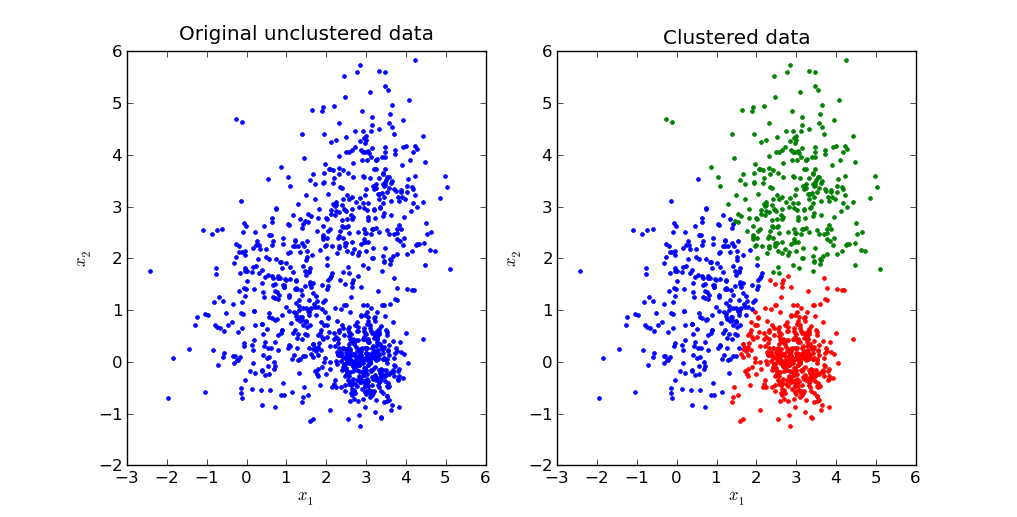
\includegraphics[width=\textwidth]{pictures/k-means-clustering}
\caption{Example of K-Means clustering algorithm results.\\
Source: \url{https://i.stack.imgur.com/cIDB3.png}}
\label{fg:k-means-clustering}
\end{figure}
K-Means clustering has linear complexity $O(n)$, thus it is considered a fast clustering algorithm.


\subsection{Non-Negative Matrix Factorization (NMF)}

Non-Negative matrix factorization is a set of algorithms for high dimensional data analysis that extract features from a set of non-negative vectors. It was first introduced by an article by Paatero and Tapper in 1994 \cite{10.1002/env.3170050203} and has been widely used ever since it was made popular by Lee and Seung in 1999 \cite{10.1038/44565}, with the first simple algorithm.\\
It has been proved empirically by different experiments \cite{10.5555/1005332.1044709, 10.1109/CVPR.2001.990477} that NMF has clustering effects.
Given a matrix $X$ with shape $m \times n$, the goal of NMF is to compute matrices $F$, with shape $m \times p$, and $G$, with shape $p \times n$, such that:
\begin{equation*}
X = FG
\end{equation*}
by solving the optimization problem:
\begin{equation*}
\min_{F \in \mathbb{R}^{m \times p}_+, G \in \mathbb{R}^{n \times p}_+} \norm{X - FG}_F^2
\end{equation*}
where $\norm{X - FG}_F^2$ is the Frobenius norm, defined as:
\begin{equation*}
\norm{X - FG}_F^2 = \sum_{i,j} (X - FG)_{i,j}^2
\end{equation*}
The standard NMF algorithm is the following:
\vskip 0.7cm
\begin{algorithm}[H]
\SetKwInOut{Input}{Input}
\SetKwInOut{Output}{Output}
\Input{Non-negative matrix $X \in \mathbb{R}^{m \times n}_+$ and factorization rank $r$.}
\Output{$(F,G) \geq 0$ : A rank-$r$ NMF of $X \approx FG$.}
Generate initial matrices $F^{(0)} \geq 0$, $G^{(0)} \geq 0$\;
\For{$t \gets 1$ \KwTo $max\_iteration$}{
  $G^{(t)} \gets G^{(t - 1)} \odot \frac{(F^{(t - 1)})^T X}{(F^{(t - 1)})^T F^{(t - 1)} G^{(t - 1)}}$\;
  $F^{(t)} \gets F^{(t - 1)} \odot \frac{X (G^{(t)})^T}{F^{(t - 1)} G^{(t)} (G^{(t)})^T}$\;
}
\caption{The standard algorithm for NMF}
\end{algorithm}
\vskip 0.7cm
$F$ and $G$ can be initialized randomly or using some other clustering method, such as K-Means clustering.


\subsection{Orthogonal Non-Negative Matrix Tri-Factorizations (ONMTF)}

Orthogonal non-negative matrix factorizations (ONMF) is a type of NMF that, given a matrix $X$ with shape $m \times n$, computes matrices $F$, with shape $m \times p$, and $G$, with shape $n \times p$, such that:
\begin{equation*}
X = FG^T
\end{equation*}
by solving the optimization problem:
\begin{equation*}
\min_{F \in \mathbb{R}^{m \times p}_+, G \in \mathbb{R}^{n \times p}_+} \norm{X - FG^T}_F^2, \quad \text{s.t.} \quad F^TF = I
\end{equation*}
Alternatively, the $G$-orthogonal optimization problem is:
\begin{equation*}
\min_{F \in \mathbb{R}^{m \times p}_+, G \in \mathbb{R}^{n \times p}_+} \norm{X - FG^T}_F^2, \quad \text{s.t.} \quad G^TG = I
\end{equation*}
The algorithms for ONMF are the following:
\vskip 0.7cm
\begin{algorithm}[H]
\SetKwInOut{Input}{Input}
\SetKwInOut{Output}{Output}
\Input{Non-negative matrix $X \in \mathbb{R}^{m \times n}_+$ and factorization rank $r$.}
\Output{$(F,G) \geq 0$ : A rank-$r$ NMF of $X \approx FG^T$.}
Generate initial matrices $F^{(0)} \geq 0$, $G^{(0)} \geq 0$\;
\For{$t \gets 1$ \KwTo $max\_iteration$}{
  $G^{(t)} \gets G^{(t - 1)} \odot \frac{X^T F^{(t - 1)}}{G^{(t - 1)} [F^{(t - 1)}]^T F^{(t - 1)}}$\;
  $F^{(t)} \gets F^{(t - 1)} \odot \sqrt{\frac{X G^{(t)}}{F^{(t - 1)} [F^{(t - 1)}]^T X G^{(t)}}}$\;
}
\caption{The algorithm for $F$-orthogonal ONMF}
\end{algorithm}
\vskip 0.7cm
\begin{algorithm}[H]
\SetKwInOut{Input}{Input}
\SetKwInOut{Output}{Output}
\Input{Non-negative matrix $X \in \mathbb{R}^{m \times n}_+$ and factorization rank $r$.}
\Output{$(F,G) \geq 0$ : A rank-$r$ NMF of $X \approx FG^T$.}
Generate initial matrices $F^{(0)} \geq 0$, $G^{(0)} \geq 0$\;
\For{$t \gets 1$ \KwTo $max\_iteration$}{
  $G^{(t)} \gets G^{(t - 1)} \odot \sqrt{\frac{X^T F^{(t - 1)}}{G^{(t - 1)} [G^{(t - 1)}]^T X^T F^{(t - 1)}}}$\;
  $F^{(t)} \gets F^{(t - 1)} \odot \frac{X [G^{(t)}]^T}{F^{(t - 1)} [G^{(t)}]^T G^{(t)}}$\;
}
\caption{The algorithm for $G$-orthogonal ONMF}
\end{algorithm}
\vskip 0.7cm
The tri-factorizations \cite{10.1145/1150402.1150420} variant uses three factors instead of two. Given a matrix $X$ with shape $m \times n$, computes matrices $F$, with shape $m \times p$, $G$, with shape $n \times r$, and $S$, with shape $p \times r$, such that:
\begin{equation*}
X = FSG^T
\end{equation*}
by solving optimization problem:
\begin{equation*}
\min_{F \in \mathbb{R}^{m \times p}_+, G \in \mathbb{R}^{n \times r}_+, S \in \mathbb{R}^{p \times r}_+} \norm{X - F S G^T}_F^2, \quad \text{s.t.} \quad F^TF = I, G^TG = I
\end{equation*}
where $p$ and $r$ are the amount of row and column clusters.\\
According to Ding \textit{et al} \cite{10.1145/1150402.1150420}, tri-factorization is capable of clustering rows and columns of the input matrix simultaneously.\\
The rules for updating $F$, $G$ and $S$, are according to the following algorithm:
\vskip 0.7cm
\begin{algorithm}[H]
\SetKwInOut{Input}{Input}
\SetKwInOut{Output}{Output}
\Input{Non-negative matrix $X \in \mathbb{R}^{m \times n}_+$ and factorization rank $r$.}
\Output{$(F,G,S) \geq 0$ : A rank-$r$ NMF of $X \approx FSG^T$.}
Generate initial matrices $F^{(0)} \geq 0$, $G^{(0)} \geq 0$, $S^{(0)} \geq 0$\;
\For{$t \gets 1$ \KwTo $max\_iteration$}{
  $G^{(t)} \gets G^{(t - 1)} \odot \sqrt{\frac{X^T F^{(t - 1)} S^{(t - 1)}}{G^{(t - 1)} [G^{(t - 1)}]^T X^T F^{(t - 1)} S^{(t - 1)}}}$\;
  $F^{(t)} \gets F^{(t - 1)} \odot \sqrt{\frac{X G^{(t)} [S^{(t - 1)}]^T}{F^{(t - 1)} (F^{(t - 1)})^T X G^{(t)} [S^{(t - 1)}]^T}}$\;
  $S^{(t)} \gets F^{(t - 1)} \odot \sqrt{\frac{[F^{(t)}]^T X G^{(t)}}{[F^{(t)}]^T F^{(t)} S^{(t - 1)} [G^{(t)}]^T G^{(t)}}}$\;
}
\caption{The algorithm for ONMTF}
\end{algorithm}



\section{Cross-Domain Recommender Systems}

While the majority of recommender systems provide recommendation targeted only to a single topic, in recent years large digital service companies like Amazon or Google started providing recommendation across a very eterogeneous set of services. Amazon, for example, provides recommendations both for its e-commerce website, for items of all categories, and for music, movies and so on. In this scenario it may be useful to provide recommendations across different domains.\par
Cross-domain recommender systems aim to generate higher quality recommendations in a target domain by leveraging data coming from one or more different source domains. In particular, knowledge acquired in a source domain can be transferred with some knowledge-transfer technique to the target domain (\autoref{fg:knowledge-transfer}).\\
\begin{figure}[hbt]
\centering
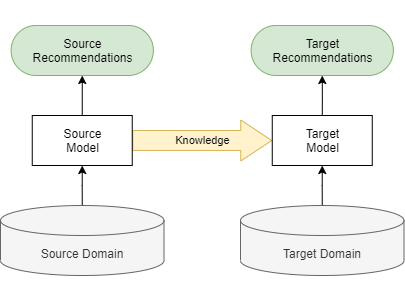
\includegraphics[width=0.8\textwidth]{pictures/knowledge-transfer}
\caption{General approach of knowledge transfer techniques.}
\label{fg:knowledge-transfer}
\end{figure}
The use cases for such approach are mainly two. First, building a user profile across domains allows to generate bundle recommendation \cite{10.1007/s11257-012-9131-2, 10.1007/s11257-007-9042-9, 10.1007/s11257-012-9128-x}. For example, it may be possible to recommend the movie transposition of a book the user bought and then to recommend the movie soundtrack. A recommendation like that can only be inferred by exploiting data from multiple domains. The second scenario is the one of the cold start problem \cite{10.1145/2645710.2645777, 10.1007/978-3-642-22362-4_26, 10.1145/2507157.2507206}. Auxiliary source domains may be able to provide information which is missing in the target domain. Both of these scenarios assume that there are correspondences between user and item profiles across domains.\par
A complete review of recommender systems was given by Cremonesi \textit{et al} \cite{10.1007/978-1-4899-7637-6_27}. To introduce their properties and categories we mainly follow their formalization of the problem.


\subsection{Domain Definitions}

The first step in introducting cross-domain recommender systems, is defining the concept of domain. We can distinguish four different levels of domain definition:
\begin{itemize}
\item \textbf{Attribute level}: two items are considered to belong to different domains if they differ in some attribute. For example two books could be considered of different domains if they differ by genre. The attribute level definition is too weak to be considered for cross-domain recommender systems.
\item \textbf{Type level}: two items are considered to belong to different domains if they share some attributes but differ by others. For example, TV series and movies belong to different domains, according to this definition.
\item \textbf{Item level}: two items are considered to belong to different domains if they do not share any attribute, or at least very few. For example, movies and books belong to different domains, according to this definition.
\item \textbf{System level}: two items are considered to belong to different domains if they belong to different systems, even if they share the same attributes. For example, movies from the Netflix system and movies from the Amazon system belong to different domains, according to this definition.
\end{itemize}


\subsection{Types of recommendation}

The goal of cross-domain recommender systems can also vary depending on which domain is the target for recommendations.\\
According to Cremonesi \textit{et al} \cite{10.1007/978-1-4899-7637-6_27}, we can distinguish three types of recommendations. Given the target domain $D_T$ with its user and item sets, respectively $U_T$ and $I_T$, and one or more source domains $D_S$ with their user and item sets, respectively $U_S$ and $I_S$, we distinguish the following recommendation types:
\begin{itemize}
\item \textbf{Multi-domain recommendation}: recommend items in $I_S \cup I_T$ to users in $U_S$ or to users in $U_T$. This approach requires a significant amount of user overlap between domains, but it is becoming feasible due to the amount of profiles maintained by users on different social media, connected by mechanisms of cross-authentication and identification \cite{10.1016/j.ins.2008.08.022} or interoperability \cite{10.1007/s11257-011-9097-5}.
\item \textbf{Linked-domain recommendation}: recommend items in $I_T$ to users in $U_S$ or $U_T$ by exploiting knowledge about $U_S \cup U_T$ and $I_S \cup I_T$. This approach is used to enrich data in a target domain with a cold start or data sparsity problem. Generally, it requires at least a partial amount of user or item overlap between the source and target domains.
\item \textbf{Cross-domain recommendation}: recommend items in $I_T$ to users in $U_S$ or $U_T$ by exploiting knowledge about $U_S$ and $I_S$. This approach is used when the target domain has no information about the users. In this scenario there is no assumption of data overlap between domains and the approaches aim at transferring knowledge from one domain to the other.
\end{itemize}


\subsection{Types of Overlap}

We can make distinction between four types of overlap (\autoref{fg:types-of-overlap}):
\begin{itemize}
\item \textbf{No overlap}: neither the user nor the item sets share common data, such that:
\begin{equation*}
U_T \cap U_S = \emptyset \quad \text{and} \quad I_T \cap I_S = \emptyset
\end{equation*}
\item \textbf{User overlap}: only the user sets share common data, such that:
\begin{equation*}
U_T \cap U_S \neq \emptyset \quad \text{and} \quad I_T \cap I_S = \emptyset
\end{equation*}
\item \textbf{Item overlap}: only the item sets share common data, such that:
\begin{equation*}
U_T \cap U_S = \emptyset \quad \text{and} \quad I_T \cap I_S \neq \emptyset
\end{equation*}
\item \textbf{User and item overlap}: both user and item sets share common data, such that:
\begin{equation*}
U_T \cap U_S \neq \emptyset \quad \text{and} \quad I_T \cap I_S \neq \emptyset
\end{equation*}
\end{itemize}
\begin{figure}[hbt]
\centering
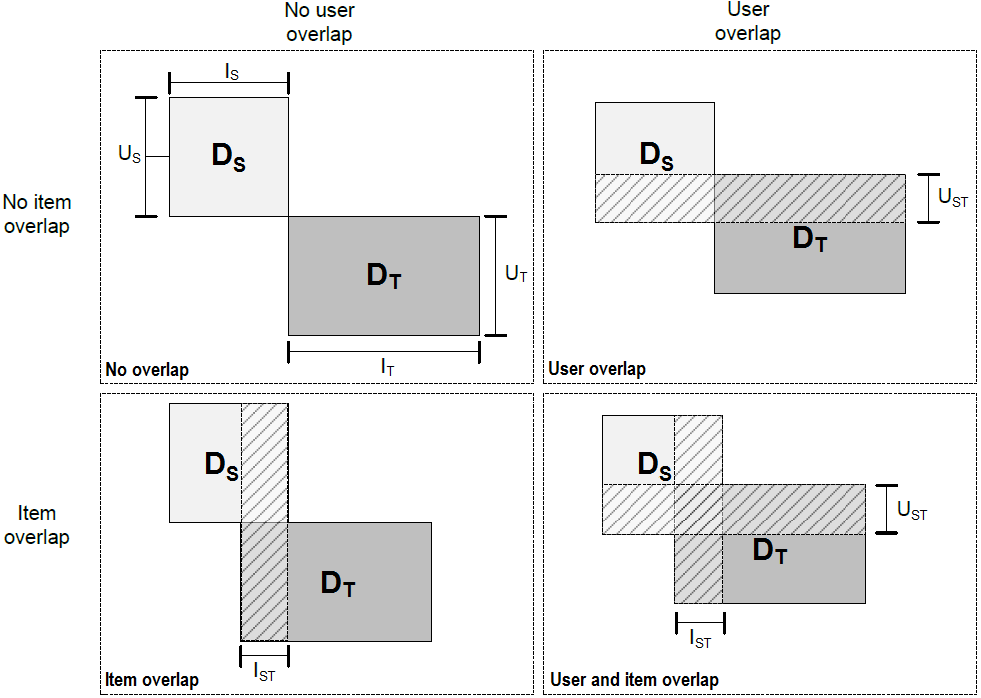
\includegraphics[width=\textwidth]{pictures/domains-overlap}
\caption{Types of overlap of user and item sets between two domains. \cite{10.1007/978-1-4899-7637-6_27}}
\label{fg:types-of-overlap}
\end{figure}


\subsection{Systems Categories}

Given the previous attributes, different cross-domain recommender system trends have been defined into a categorization by Loizou \cite{crossdomain-recsys-categorization}, which was later enhanced by Cremonesi \textit{et al} \cite{crossdomain-recsys-categorization} into four groups:
\begin{itemize}
\item As proposed by Lee \cite{10.1016/S0957-41740100034-3}, extract association rules from rating behavior in source domains, to be used in the target domain.
\item As proposed by Cao \textit{et al.} \cite{10.5555/3104322.3104344} and Zhang \textit{et al.} \cite{10.5555/3023549.3023635}, learn inter-domain similarity based on ratings and correlation matrices.
\item As proposed by Zhuang \textit{et al.} \cite{10.1109/TKDE.2009.205}, combine estimations of rating probability distributions in source domains, to be used in the target domain.
\item As proposed by Li \textit{et al.} \cite{10.5555/1661445.1661773, 10.1145/1553374.1553454} and Pan \textit{et al.} \cite{10.5555/2283696.2283784, 10.5555/2898607.2898644}, transfer knowledge from source domains to the target domain to reduce rating sparsity.
\end{itemize}
Furthermore, it is possible to make another type of distinction based on the approach of knowledge exploitation, into two macro-groups and sub-groups (\autoref{fg:types-of-knowledge-exploitation}).
\begin{figure}[hbt]
\centering
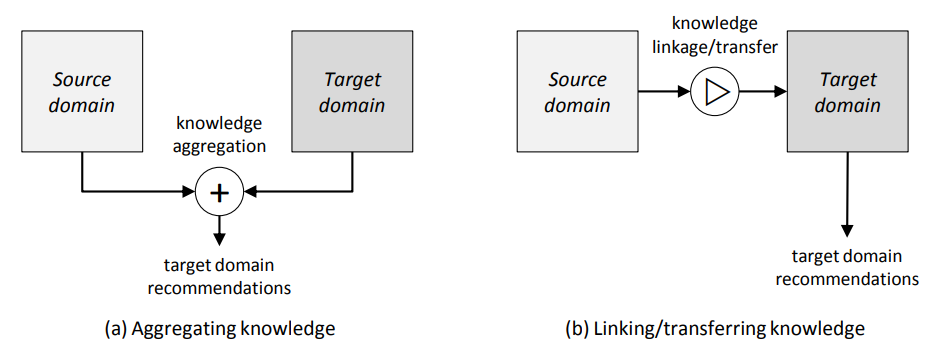
\includegraphics[width=\textwidth]{pictures/knowledge-exploitation}
\caption{Types of knowledge exploitation in cross-domain recommender systems. \cite{10.1007/978-1-4899-7637-6_27}}
\label{fg:types-of-knowledge-exploitation}
\end{figure}
\begin{itemize}
\item \textbf{Aggregating knowledge}
\begin{itemize}
\item \textbf{\textit{Merging user preferences}}: the aggregated knowledge consists of user preferences. Combining user profiles from multiple domains requires a single type of representation of user preferences.\\
This is the most used approach for cross domain recommendation. According to multiple sources \cite{10.1007/s11257-012-9131-2, 10.1007/978-3-540-88564-1_40, 10.1007/978-3-540-73078-1_44, 10.1145/1297231.1297238, 10.1007/s00354-008-0041-0}, by having user overlap between multiple domains and significant information about user preference in each domain, it is possible to extract a more complete user profile, to provide better recommendations with higher accuracy, by combining the user preferences in a single multi-domain profile. The aggregation of user preferences is able to provide knowledge about user tastes that cannot be extracted from a single domain.\\
According to others, aggregating user preferences is also beneficial to address the problem of cold-start \cite{10.1007/978-3-642-38844-6_25} and data sparsity \cite{10.1007/s11257-012-9128-x}.\\
While merging user preferences as ratings has proved the be the most efficient approach of building a multi-domain user profile, in real scenarios it is rarely possible to achieve a common represantion for ratings and to provide a sufficient user overlap. Thus, more recent methods have focused on aggregating user tags. According to Szomszor \textit{et al.} \cite{10.1145/1379092.1379103, 10.1007/978-3-540-88564-1_40} it is possible to obtain higher quality recommendations by aggregating and correlating user social tags between domains. Such approach does not require user overlap.
\item \textbf{\textit{Mediating user modeling data}} (\autoref{fg:mediating-user-modeling-data}): the aggregated knowledge consists of user models, such as similarities or neighbors.\\
This approach extends the previous one by aggregating information related to models of users and items. According to Berkovsky et al. \cite{10.1007/s11257-007-9042-9, 10.1007/11590323_22} this approach enriches the user model and allows to provide higher quality recommendations in each aggregated domain.\\
For example, with the assumption of user overlap between domains, it is possible to merge the lists of user neighbors \cite{10.1145/1297231.1297238}. The same approach can be applied to item models.
\item \textbf{\textit{Combining single domain recommendations}} (\autoref{fg:combining-single-domain-recommendations}): the aggregated knowledge is composed of single-domain recommendations.\\
In this approach, recommendations made in the source domains are used to enrich the recommendations in the target domain. Aggregating user recommendations requires both user and item overlap. While the recommendations in the single domains can be computed with different approaches, the challenge of this scenario is to compute weights for aggregation.
\end{itemize}
\item \textbf{Linking and transferring knowledge}:
\begin{itemize}
\item \textbf{\textit{Linking domains}} (\autoref{fg:linking-domains}): source and target domains are linked by common knowledge, such as item attributes.\\
This correspondences can either be directly identified between the single domains or with the aid of an external domain. Despite no user or item overlap being needed for this approach, at least a partial feature overlap is required.\\
Chung \textit{et al.} \cite{10.1145/1282100.1282113} initially proposed an approach using item attributes directly to identify a bridge between domains, but since items are generally very heterogeneus, it may be difficult to find directly corresponding features. To address this problem, Loizou \cite{crossdomain-recsys-categorization} proposed to use Wikipedia as a universal vocabulary to express and relate user preferences across multiple domains.\\
The known problem of both approaches is building said knowledge repositories. Cremonesi \textit{et al.} \cite{10.1007/978-1-4899-7637-6_27} observed that the majority of approaches with the goal of linking domains does not require user or item overlap, but only feature overlap between domains. It was also observed that no particular approach outperforms the others in a general scenario.
\item \textbf{\textit{Sharing latent features}} (\autoref{fg:sharing-latent-features}): source and target domains are linked by common latent features, such as extracted item features.\\
This approach is similar to the previous one, although it assumes that using denser representations of user preferences or item attributes, which are usually both very sparse sets, leads to more accurate matches \cite{10.5555/2283696.2283784, 10.5555/2898607.2898644}. These new representations are obtained with various factorization algorithms. Like for the previous approach, at least a feature overlap is strictly needed.
\item \textbf{\textit{Transferring rating patterns}} (\autoref{fg:transferring-rating-patterns}): the rating pattern extracted from one or more source domains is transferred and applied in the target domain.\\
The base assumption of this approach is that similar domains share the population used to sample user preferences, even if there is no user or item overlap between them. For this reason it may be possible to find a correlation between domains of the preferences of groups of users for groups of items. This correlation is called \textit{rating pattern}. Thus, the rating pattern is the only information transferred from source domains to the target domain.\\
The first approach that aims to transfer the rating pattern between domains was proposed by Li \textit{et al.} \cite{10.5555/1661445.1661773} and named \textit{codebook transfer}. Since then, several variants of codebook transfer have surfaced, all based on the same assumptions.\\
Being the focus of this thesis for evaluation purposes, the details of the codebook transfer theoretical model and its extensions are addressed in \autoref{ch:analysed-models}.
\end{itemize}
\end{itemize}
Since in this thesis we evaluate the codebook transfer technique, we focus on transferring knowledge and, in particular, on transferring rating patterns.

\begin{figure}[H]
\centering
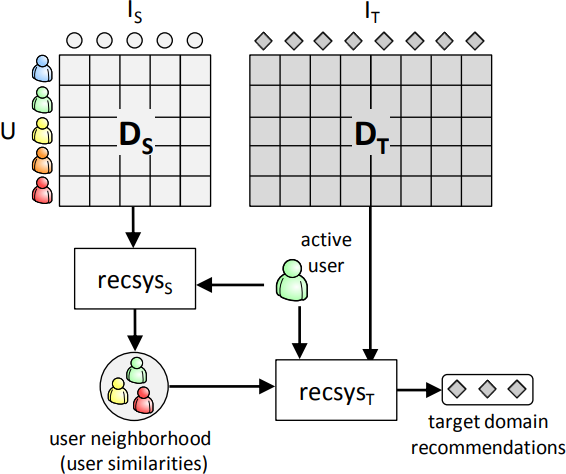
\includegraphics[width=0.8\textwidth]{pictures/mediating-user-modeling-data}
\caption{Representation of the \textit{mediating user modeling data} approach. \cite{10.1007/978-1-4899-7637-6_27}}
\label{fg:mediating-user-modeling-data}
\end{figure}
\begin{figure}[H]
\centering
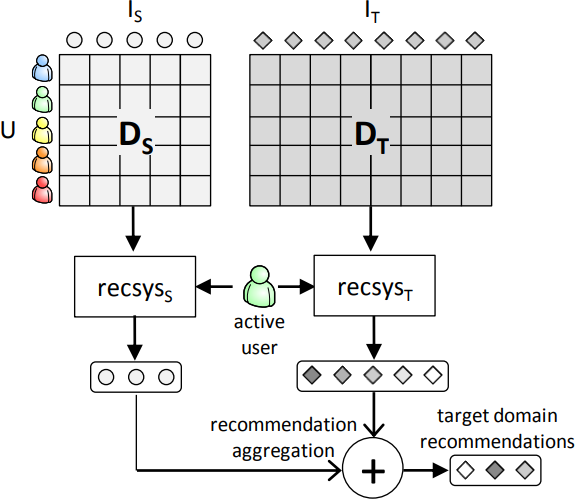
\includegraphics[width=0.8\textwidth]{pictures/combining-single-domain-recommendations}
\caption{Representation of the \textit{combining single domain recommendations} approach. \cite{10.1007/978-1-4899-7637-6_27}}
\label{fg:combining-single-domain-recommendations}
\end{figure}
\begin{figure}[H]
\centering
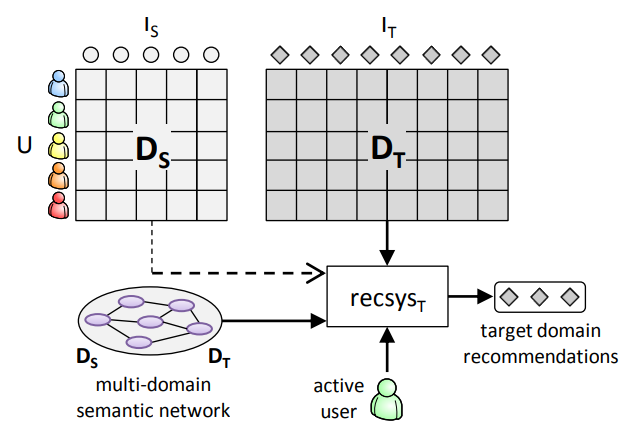
\includegraphics[width=0.8\textwidth]{pictures/linking-domains}
\caption{Representation of the \textit{linking domains} approach. \cite{10.1007/978-1-4899-7637-6_27}}
\label{fg:linking-domains}
\end{figure}
\begin{figure}[H]
\centering
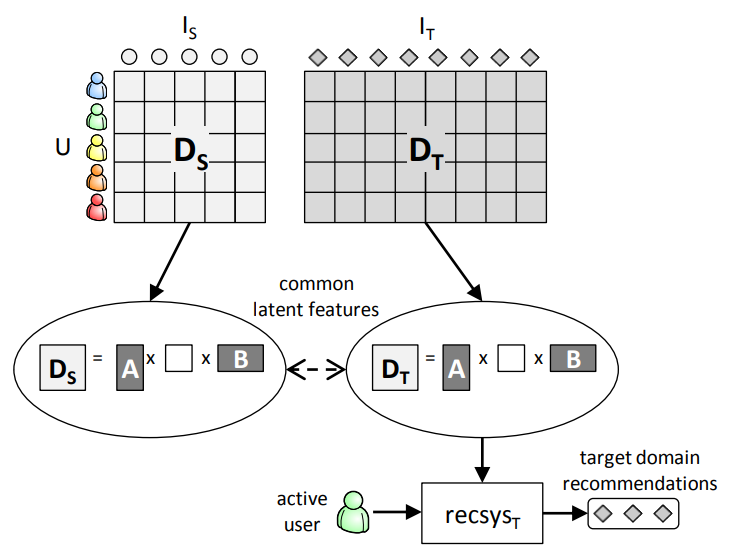
\includegraphics[width=0.8\textwidth]{pictures/sharing-latent-features}
\caption{Representation of the \textit{sharing latent features} approach. \cite{10.1007/978-1-4899-7637-6_27}}
\label{fg:sharing-latent-features}
\end{figure}
\begin{figure}[H]
\centering
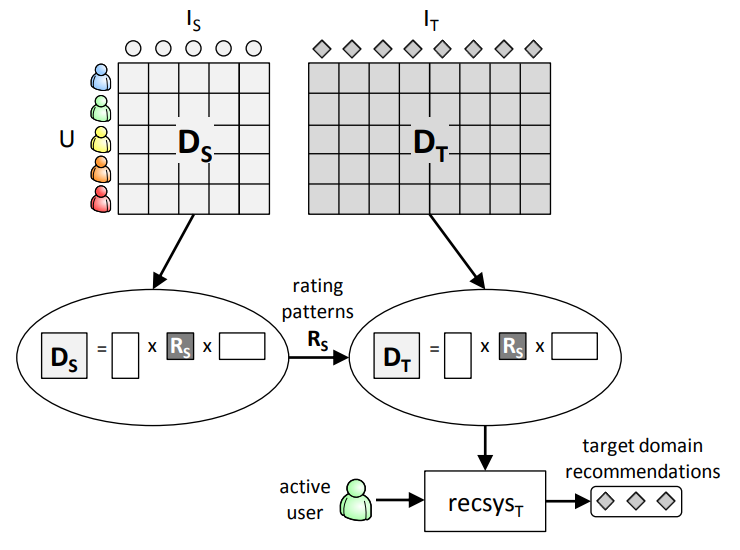
\includegraphics[width=0.8\textwidth]{pictures/transferring-rating-patterns}
\caption{Representation of the \textit{transferring rating patterns} approach. \cite{10.1007/978-1-4899-7637-6_27}}
\label{fg:transferring-rating-patterns}
\end{figure}



\section{The Problem of Rating Pattern Transfer Without Overlap}

In 2014, Cremonesi and Quadrana \cite{10.1145/2645710.2645769} performed experiments on codebook transfer to evaluate its performance in rating prediction. According to them, codebook transfer is not able to transfer knowledge between non-overlapping domains. In their experiments, they provide an alternative explaination based on three points to the apparent increase of accuracy obtained with codebook transfer:
\begin{itemize}
\item Empirical proof that CBT can improve accuracy without transferring knowledge.
\item The injection of the codebook in the target domain is equivalent to a two-matrix factorization algorithm without transfer of knowledge from the source domain.
\item The apparent increase of accuracy is due to a pitfall in the evaluation procedure, as it compares a user-based kNN algorithm (before the injection) with a matrix factorization algorithm (after the injection) and matrix factorization is known to outperform kNN.
\end{itemize}
Expanding on the issue raised by Cremonesi and Quadrana in the rating prediction task, in this thesis we provide a ranking evaluation of two codebook transfer approaches, described in \autoref{ch:analysed-models}.